\documentclass[12pt,a4paper]{extreport}
\usepackage[l2tabu,orthodox]{nag}
\usepackage[left=10mm,right=50mm, top=15mm,bottom=15mm,bindingoffset=0cm]{geometry}
\usepackage{indentfirst}

\usepackage{ccaption}
\captiondelim{. }

\usepackage{amssymb,amsfonts}
\usepackage{cmap}
\usepackage[T2A]{fontenc}
\usepackage[utf8]{inputenc}
\usepackage{ucs}
\usepackage[russian,english]{babel}
\usepackage[babel = true]{microtype}
\usepackage{graphicx}
\graphicspath{{img/}}
\DeclareGraphicsExtensions{.pdf,.png,.jpg}


\usepackage{color}
\definecolor{darkblue}{rgb}{0,0,.75}
\definecolor{darkred}{rgb}{.7,0,0}
\definecolor{darkgreen}{rgb}{0,.7,0}

\usepackage[normalem]{ulem}
\usepackage[textwidth=4cm,textsize=tiny]{todonotes}
\newcommand{\fix}[2]{{\textcolor{red}{\uwave{#1}}\todo[fancyline]{#2}}}
\newcommand{\hl}[1]{{\textcolor{red}{#1}}}
\newcommand{\cmd}[1]{{\ttfamily{\textbackslash #1}}}
\usepackage[pverb-linebreak=no]{examplep}
\newcommand{\vrb}[1]{\PVerb{#1}}
\newcommand{\vrbb}[1]{\texttt{\textbackslash}\PVerb{#1}}
\newcommand{\rulez}{{\href{https://goo.gl/FhyJJm}{Правила}}}


\usepackage{listings}
    \lstnewenvironment{python}{\lstset{language=Python,
    tabsize=4,
    basicstyle=\footnotesize\ttfamily,
    stringstyle=\color{darkgreen},
    commentstyle=\color{darkred},
    keywordstyle=\color{darkblue},
    mathescape=true,
    showstringspaces=false,
    xleftmargin=.04\textwidth}}{}

\usepackage[ruled,vlined]{algorithm2e}

\usepackage[
    draft = false,
    unicode = true,
    colorlinks = true,
    allcolors = blue,
    hyperfootnotes = true
]{hyperref}

\usepackage{amsmath}

\usepackage{amsthm}
    \theoremstyle{plain}
    \newtheorem{theorem}{Теорема}
    \newtheorem{lemma}{Лемма}
    \newtheorem{proposition}{Утверждение}
    \newtheorem{corollary}{Следствие}
    \theoremstyle{definition}
    \newtheorem{definition}{Определение}
    \newtheorem{notation}{Обозначение}
    \newtheorem{example}{Пример}

\newenvironment{task}[1]
    {\par\noindent\textbf{Задача \href{http://progensys.dainiak.com/problem-#1}{#1}. }}
    {\smallskip}
\newenvironment{solution}
    {\par\noindent\textbf{Решение. }}
    {\bigskip}

\title{Решения задач по курсу «Дискретные структуры»}
\author{Антон Никишин}

\begin{document}
\maketitle

% Таким образом нужно добавлять решения задач:
\begin{task}{314}
\begin{enumerate}
\item Какое количество ребер может быть в пятивершинном порожденном подграфе полного десятивершинного графа?
\item Какое максимальное количество ребер может быть в остовном подграфе полного десятивершинного графа?
\item Как могла бы выглядеть «теорема о рукопожатиях» для гиперграфов?
\item В графе $G$ имеется $3k$ изолированных вершин, $2m$ висячих вершин, $n$ проходных вершин, а других вершин в $G$ нет. Чему равняется $\|G\|$? Ответ запишите в виде формулы от $m$, $n$, $k$.
\end{enumerate}
\end{task}

\begin{solution}
\begin{enumerate}
\item В изначальном графе между любой парой вершин было ребро, так как это $K_{10}$. Выберем любые 5 вершин в нём. Между любыми из них будет ребро. По определению порождённого подграфа имеем, что любой порождённый пятивершинный граф из $K_{10}$ будет изоморфен $K_5$. Получается, что его число рёбер $\frac{5(5-1)}{2}=10$.
\item Остовный подграф содержит все вершины исходного графа и часть из его рёбер. Очевидно, максимальное значение будет достигаться, когда в остовный подграф войдут все рёбра, $\frac{10(10-1)}{2}=45$.
\item Было решено.
\item По теореме о рукопожатиях удвоенное число рёбер равно сумме степеней вершин. Получаем ответ: $\frac{0 \cdot 3k+1 \cdot 2m+2 \cdot k}{2}=m+k$
\end{enumerate}
\end{solution}
\begin{task}{73}
Квадратная таблица $(2n+1)\times(2n+1)$, где $n\in\mathbb{N}$, заполнена числами от $1$ до $2n+1$ так, что в каждой строке и в каждом столбце представлены все эти числа. Докажите, что если это расположение симметрично относительно диагонали таблицы, то на этой диагонали тоже представлены все эти числа. В решении используйте принцип Дирихле, обязательно явно указав все детали применения (если пользуетесь «клеточно-кроликовой» терминологией, то что в Вашей задаче играет роль «клеток» и что — роль «кроликов»; если более строгой формулировкой, то как общая формулировка «ложится» на конкретику Вашей задачи).
\end{task}

\begin{solution}
Пусть какое-то число на диагонали встречается дважды, значит на диагонали остается $2n-1$ пустая клетка. Всего различных неиспользованных чисел остаётся $2n$ (это будут кролики). По принципу Дирихле найдётся число, которое не будет выписано на диагонали. Обозначим такое число за $k$. Если число с аналогичным значением $k$ встречается в клетке с координатами $(x, y)$, то встречается и в клетке $(y, x)$, при этом $y\neq x$. Получается, все числа со значением $k$ разбиты на не повторяющиеся пары, но чисел $k$ --- $2n+1$ штук (нечётное количество). Приходим к противоречию. Получается, что каждое число встречается на диагонали по одному разу. 
\end{solution}
\begin{task}{15}
На потоке второго курса ПМФ ФИВТ три группы. Преподаватели узнали, что каждый второкурсник ПМФ всегда даёт списывать ровно одному своему коллеге (всегда одному и тому же). Докажите, что деканат может заново перераспределить студентов по трём группам, так, что в каждой отдельной группе не окажется ни одной пары студентов, из которых один даёт списывать другому. (Перераспределяйте шаг за шагом, так, чтобы каждый шаг приводил к улучшению ситуации.) [Необходимо решить задачу непременно методом потенциалов, явно указав, какая функция используется в качестве «потенциала».]
\end{task}

\begin{solution}
В качестве потенциала будем использовать число человек, которые дают списывать одногруппнику.  Если потенциал больше нуля, то выберем любого человека, который даёт списывать одногруппнику (он очевидно найдётся). Переведём его в ту группу, в которой нет человека, который даёт ему списывать. Такая найдётся, так как число групп равно трём. При таком действии потенциал уменьшается, исходя из его определения. Будем повторять это действие пока потенциал не станет равным нулю. По достижении нуля мы выполним задачу. 
\end{solution}
\begin{task}{72}
Из двух представленных ниже графов ровно один планарен. Перерисуйте планарный граф без пересечений рёбер, а в непланарном графе найдите подграф, гомеоморфный $K_{3,3}$.

\begin{center}
  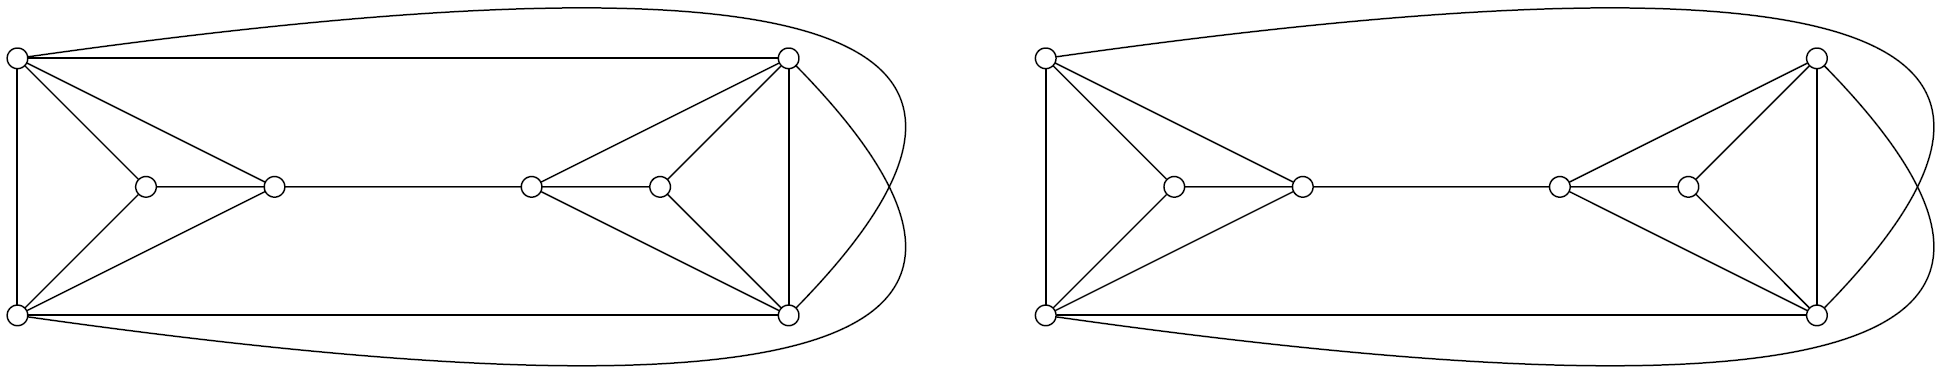
\includegraphics[width=0.8\linewidth]{72_1}
\end{center}
\end{task}

\begin{solution}
Выделим в первом графе $K_{3,3}$. По теореме Понтрягина — Куратовского он непланарный.
\begin{center}
  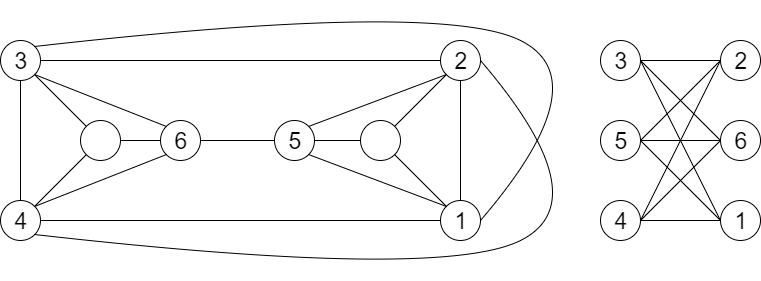
\includegraphics[width=0.8\linewidth]{72_2}
\end{center}
Перерисуем второй граф. Как видно, он планарный.
\begin{center}
  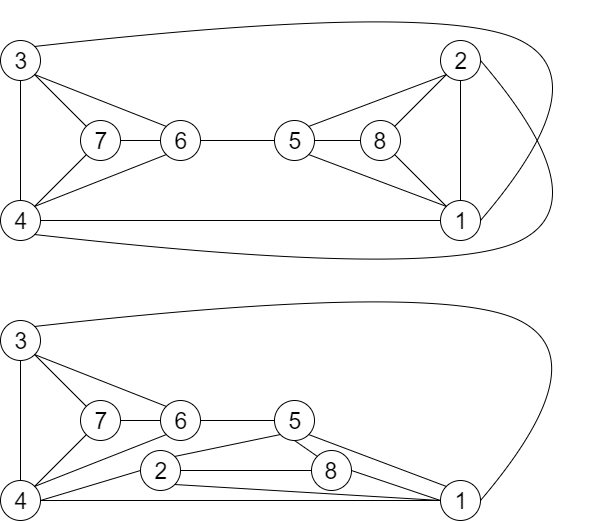
\includegraphics[width=0.6\linewidth]{72_3}
\end{center}
\end{solution}
\begin{task}{318}
Сколько перестановок на множестве $\{1, 2, ... , n\}$ представимы в виде композиции чётного количества транспозиций?
\end{task}

\begin{solution}
Составим биекцию между перестановками, представимыми в виде композиции чётного и нечётного количества транспозиций.
Будем сопоставлять следующие перестановки:
\begin{center}
$
\begin{pmatrix}
 1& 2& \ldots& n\\
 a_1& a_2& \ldots& a_n
\end{pmatrix}
$
и
$
\begin{pmatrix}
 1& 2& \ldots& n\\
 a_2& a_1& \ldots& a_n
\end{pmatrix}
$
\end{center}
Если первая перестановка представима в виде чётного количества транспозиций:
\begin{center}
$
\begin{pmatrix}
 1& 2& \ldots& n\\
 a_1& a_2& \ldots& a_n
\end{pmatrix}
=
\begin{pmatrix}
 t_1& t_2
\end{pmatrix}
\cdot
\begin{pmatrix}
 t_3& t_4
\end{pmatrix}
\cdot\ldots\cdot
\begin{pmatrix}
 t_{k-1}& t_k
\end{pmatrix}
$
\end{center}
То сопоставленная ей будет иметь нечётное количество транспозиций:
\begin{center}
$
\begin{pmatrix}
 1& 2& \ldots& n\\
 a_2& a_1& \ldots& a_n
\end{pmatrix}
=
\begin{pmatrix}
 a_1& a_2
\end{pmatrix}
\cdot
\begin{pmatrix}
 t_1& t_2
\end{pmatrix}
\cdot
\begin{pmatrix}
 t_3& t_4
\end{pmatrix}
\cdot\ldots\cdot
\begin{pmatrix}
 t_{k-1}& t_k
\end{pmatrix}
$
\end{center}
Очевидно и обратное. Здесь выполняется инъективность (действительно, если образы одинаковые, то и прообразы одинаковы, т.к. они получаются перестановкой первых двух членов). Также выполняется и сюрьективность (для любой перестановки найдётся прообраз, который находится по схожему принципу). Таким образом, мы построили биекцию между перестановками, представимыми в виде композиции чётного и нечётного количества транспозиций. Тогда перестановок обоих типов одинаковое количество. Так как общее количество перестановок $n!$, то количество перестановок, представимых в виде композиции чётного количества транспозиций, равняется $\frac{n!}{2}$.
\end{solution}
\begin{task}{150}
Пусть $f, g, h$ -- неубывающие функции из $\mathbb{R^+}$ в $\mathbb{R^+}$. Пусть $n\rightarrow\infty$. Верно ли, что если $f(n)=O(g(n))$ и $g(n)=O(h(n))$, то обязательно $f(n)=O(h(n))$? Если верно, то обоснуйте, опираясь исключительно на определения. Если же не верно в общем случае, то приведите соответствующий контрпример.
\end{task}

\begin{solution}\\
$f(n)=O(g(n)) \Leftrightarrow \exists C_1 \;\exists N_1\; \forall n\geq N_1: f(n)\leq C_1 g(n)$\\
$g(n)=O(h(n)) \Leftrightarrow \exists C_2 \;\exists N_2\; \forall n\geq N_2: g(n)\leq C_1 h(n)$\\
$\Rightarrow \exists C=C_1\cdot C_2\; \exists N=\max(N_1, N_2)\;\forall n\geq N: f(n)\leq C_1 g(n)\leq C_1\cdot C_2 h(n)=Ch(n)$
$\Leftrightarrow f(n)=O(h(n))$ 
\end{solution}
\begin{task}{146}
Пусть $n\rightarrow \infty$. Найдите асимптотику полиномиального коэффициента $P(2n, 5n, n, \sqrt{n})=\frac{(8n+\sqrt{n})!}{(2n)!(5n)!n!\sqrt{n}!}$. Под нахождением асимптотики подразумевается нахождение такой функции $f$, между которой и оцениваемой величиной можно было бы составить знак $\sim$. Ответ принимается только в виде формулы, не содержащей неопределённостей вида $1^\infty, 0^0, (\text{const} + 0)^\infty$  и пр.
\end{task}

\begin{solution}
\par Для начала воспользуемся формулой Стирлинга
\begin{equation*}
    n!=\sqrt{2\pi n}\left(\frac{n}{e}\right)^{n},
\end{equation*}
получим:
\begin{align*}
    P(2n, 5n, n, \sqrt{n})
    &=\frac{(8n+\sqrt{n})!}{(2n)!(5n)!n!\sqrt{n}!}\sim\displaybreak[3]\\
    &\sim\frac{\sqrt{2\pi(8n+\sqrt{n})}\left(\frac{8n+\sqrt{n}}{e}\right)^{8n+\sqrt{n}}}{\sqrt{2\pi}^4\sqrt{2n\cdot 5n\cdot n\cdot \sqrt{n}}\left(\frac{2n}{e}\right)^{2n}\left(\frac{5n}{e}\right)^{5n}\left(\frac{n}{e}\right)^{n}\left(\frac{\sqrt{n}}{e}\right)^{\sqrt{n}}}\sim\\
    &\sim\frac{\sqrt{8n+\sqrt{n}}(8n+\sqrt{n})^{8n+\sqrt{n}}}{\sqrt{2\pi}^3\sqrt{10n^3\sqrt{n}}(2n)^{2n}(5n)^{5n}(n)^{n}(\sqrt{n})^{\sqrt{n}}}
\end{align*}
Отдельно рассмотрим чему асимптотически равняется $(8n+\sqrt{n})^{8n+\sqrt{n}}$:
\begin{align*}
    e^{(8n+\sqrt{n})\ln{(8n+\sqrt{n})}}
    &=e^{(8n+\sqrt{n})(\ln{n}+\ln{(8+\frac{1}{\sqrt{n}})})}\sim n^{8n+\sqrt{n}}e^{(8n+\sqrt{n})(\ln8+\frac{1}{8\sqrt{n}}-\frac{1}{128n} + O(n^{-1}))}\sim\\
    &\sim n^{8n+\sqrt{n}}8^{(8n+\sqrt{n})}e^{\sqrt{n}+\frac{1}{16}}
\end{align*}
Окончательно:
\begin{align*}
    P
    &\sim\frac{\sqrt{8n}n^{8n+\sqrt{n}}8^{(8n+\sqrt{n})}e^{\sqrt{n}+\frac{1}{16}}}{\sqrt{2\pi}^3\sqrt{10n^3\sqrt{n}}(2n)^{2n}(5n)^{5n}(n)^{n}(\sqrt{n})^{\sqrt{n}}}=\\
    &=\frac{n^{8n+\sqrt{n}+\frac{1}{2}-\frac{7}{4}-2n-5n-n-\frac{\sqrt{n}}{2}}2^{24n+3\sqrt{n}+\frac{3}{2}-\frac{3}{2}-2n}e^{\sqrt{n}+\frac{1}{16}}}{\sqrt{10\pi^3}5^{5n}}=\\
    &=\frac{n^{\frac{\sqrt{n}}{2}-\frac{5}{4}}2^{22n+3\sqrt{n}}e^{\sqrt{n}+\frac{1}{16}}}{\sqrt{10\pi^3}5^{5n}}
\end{align*}
\end{solution}
\begin{task}{322}
Пусть $n$ — произвольное натуральное число. Пусть $S_1, \dots, S_{n^{2017}}$ — произвольные $n$‑элементные множества. Докажите, что при всех достаточно больших значениях $n$ можно покрасить элементы в красный и синий цвета, так, чтобы в каждом из множеств $S_i$ нашёлся хотя бы один красный и хотя бы один синий элемент.
\end{task}

\begin{solution}
Покрасим элементы множеств независимо друг от друга в два цвета (красный и синий) с одинаковой вероятностью. Тогда вероятность обоих событий равна $\frac{1}{2}$. По условию нужно показать, что
\begin{equation*}
    P(\text{в каждом }S_i\text{ есть элементы обоих цветов})>0.
\end{equation*}
Это эквивалентно доказательству того, что
\begin{equation}\label{P(A)}
    P(A)\equiv P(\exists S_i\text{, элементы которого покрашены в один цвет})<1.
\end{equation}
Отдельно рассмотрим следующий случай:
\begin{align}\label{P(A_i)}
    P(A_i)
    &\equiv P(S_i\text{ покрашен в один цвет})=\nonumber \\
      &=P(S_i\text{ покрашен полностью в красный})+\nonumber \\
      &\qquad+P(S_i\text{ покрашен полностью в синий})=\nonumber\\
    &=\left(\frac{1}{2}\right)^n+\left(\frac{1}{2}\right)^n=\left(\frac{1}{2}\right)^{n-1}.
\end{align}
Покажем, что \eqref{P(A)} выполняется, воспользовавшись результатом \eqref{P(A_i)}.
\begin{equation}\label{result}
    P(A)=P\left(\bigcup_{i = 1}^{n^{2017}}A_i\right)\leq\sum_{i = 1}^{n^{2017}}P(A_i)=\frac{n^{2017}}{2^{n-1}}
\end{equation}
Выполним предельный переход в \eqref{result}.
\begin{equation*}
    P(A)=2^{2017\log{n}+1-n}\xrightarrow{n\rightarrow \infty} 0
\end{equation*}
Таким образом, мы доказали \eqref{P(A)} и получили, что при достаточно больших значениях $n$ существует раскраска, где в каждом $S_i$ найдутся элементы обоих цветов. 
\end{solution}

\begin{task}{320}
Опишите все элементы $x$ симметрической группы $\mathbb{S}_n$, для которых $x^3=e$, где $e$ — нейтральный элемент группы.
\end{task}

\begin{solution}
Будем исходить из того, что перестановка представима в виде композиции \textbf{непересекающихся} циклов (в том числе и длины один). Рассмотрим циклы $c_k$ длины $k\geq1$.
\begin{enumerate}
    \item При $k=1$ цикл является тождественной перестановкой, значит он нам подходит (действительно, $e^3=e$).
    \item При $k=2$ получаем $c_2^3=(c_2\cdot c_2)\cdot c_2=e\cdot c_2=c_2\neq e$.
    \item При $k=3$ имеем $c_3^3=e$.
    \item При больших значениях $k$ цикл <<не успеет>> довести элементы до начального положения.
\end{enumerate}
Таким образом, получаем, что под условие подходят только циклы длины один и три, а подходящие элементы группы являются композициями этих непересекающихся циклов.
\end{solution}
\begin{task}{307}
Дан клетчатый прямоугольник размером $n\times 2, n\in \mathbb{N}$. Обозначим символом $a_n$ число способов замостить этот прямоугольник фигурами двух типов: уголками размером $2\times 3$ и доминошками размера $3\times 1$ (см. рис. 1). Никакие две фигуры не должны перекрываться и каждая клетка прямоугольника должна быть покрыта некоторой фигурой. Выведите линейное рекуррентное соотношение для $a_n$ и вычислите значения $a_1,  a_2, a_3, a_4, a_5, \text{и } a_6$. Замощения, совмещающиеся отражениями относительно обеих осей симметрии прямоугольника, считаются различными. Считайте, что $a_0=1$. Пример замощения прямоугольника размера $7\times 2$ приведён на рис.2.
\begin{center}
  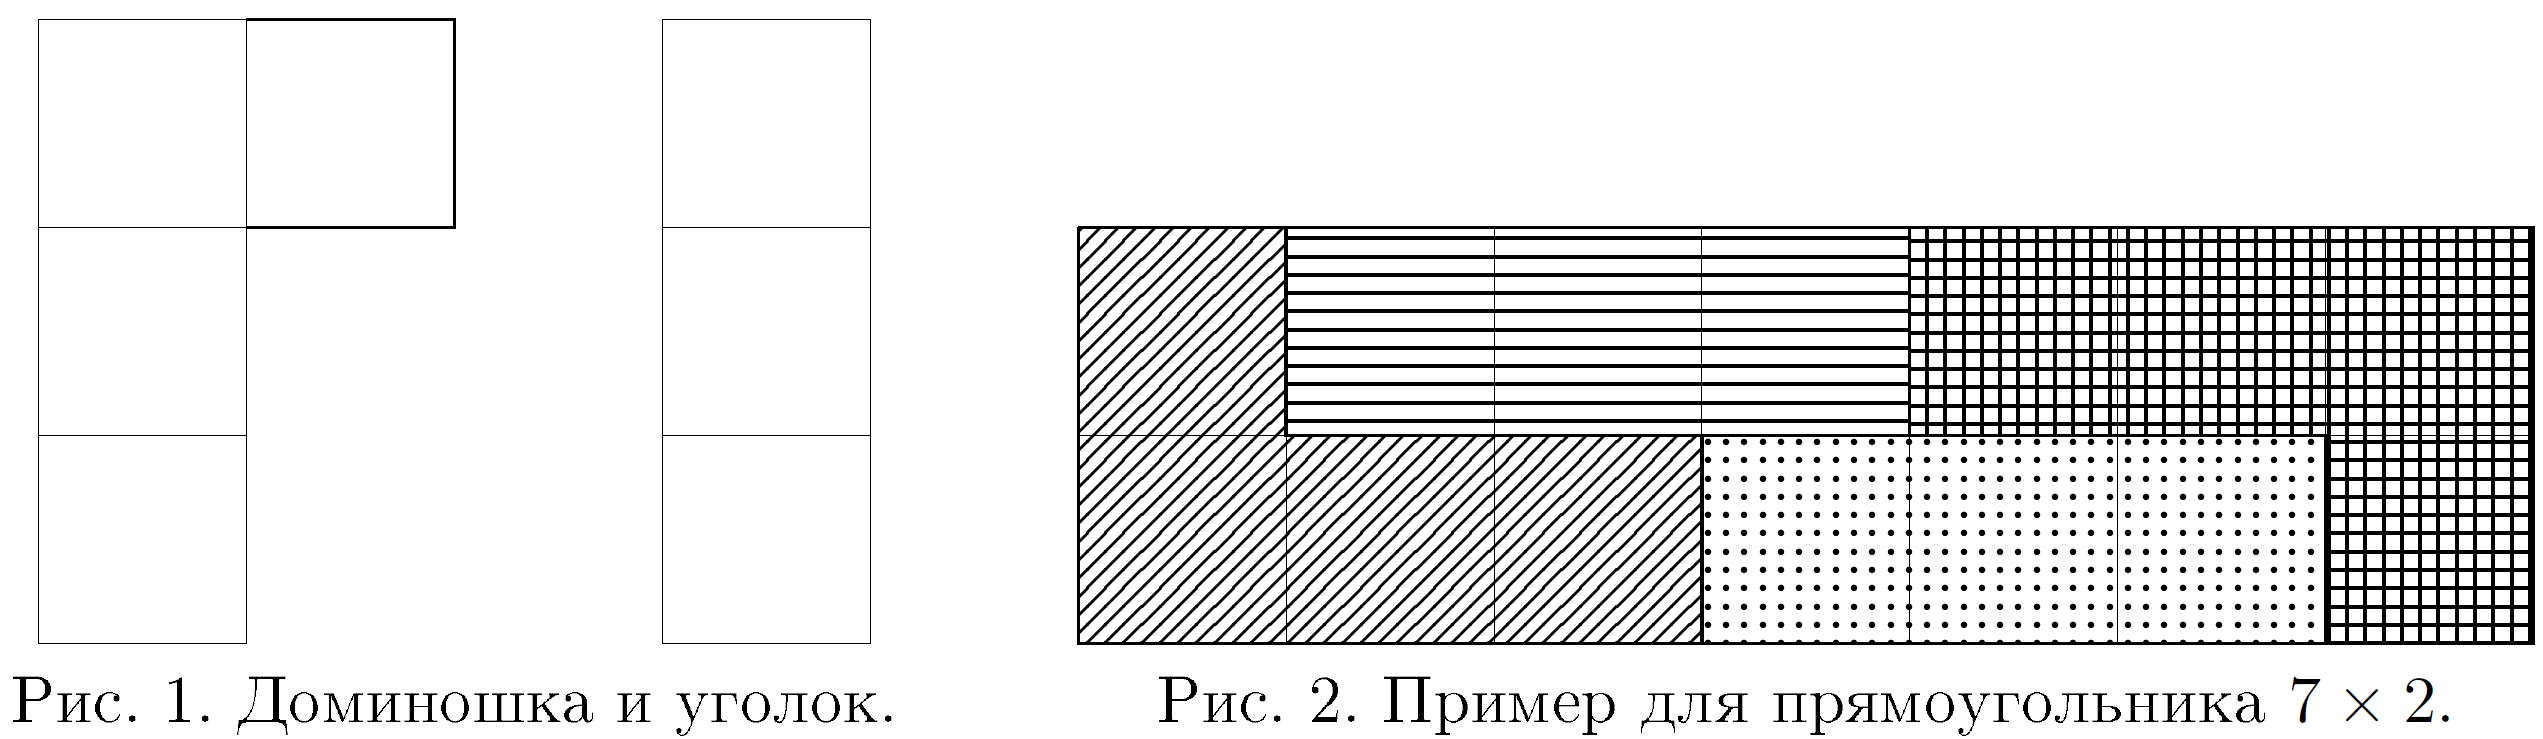
\includegraphics[width=0.65\linewidth]{307_1}
\end{center}
\end{task}

\begin{solution}
Положим в левый верхний угол фигурку и рассмотрим дальнейшие варианты замощения.
\begin{center}
  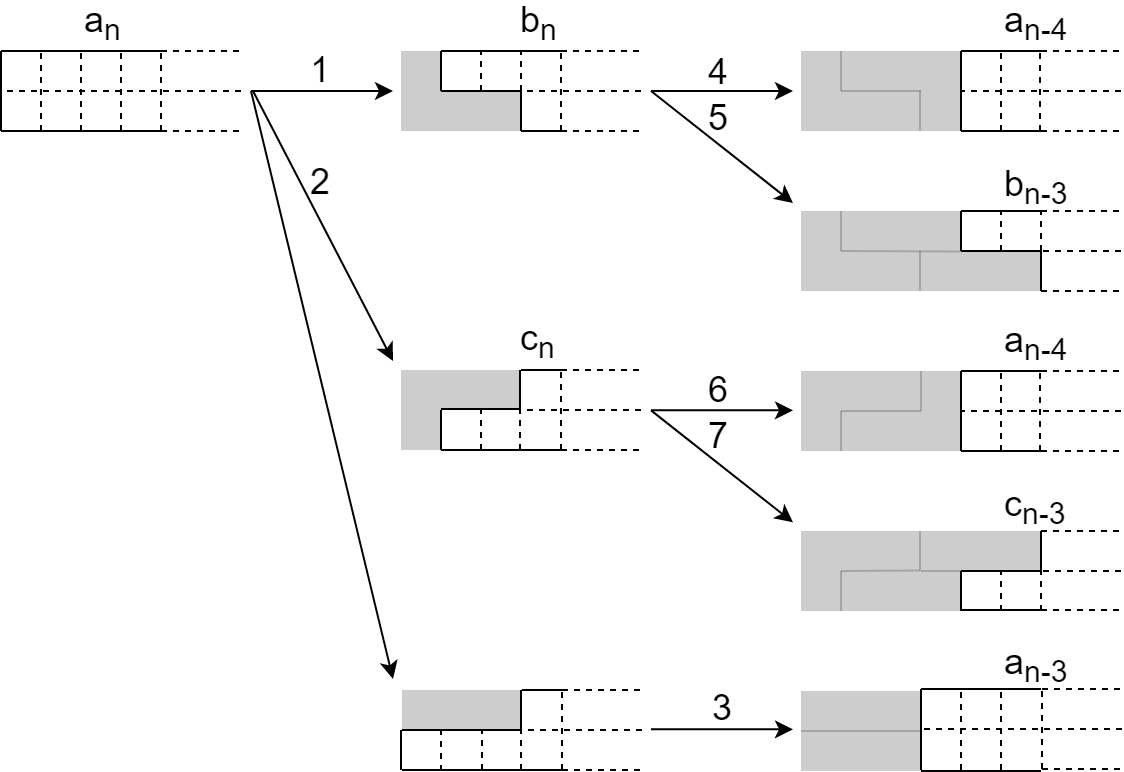
\includegraphics[width=0.65\linewidth]{307_2}
\end{center}
Составим систему уравнений, опираясь на переходы, отмеченные на схеме.
\[
\begin{cases}
    a_n=b_n+c_n+a_{n-3} &\text{из 1, 2 и 3}\\
    b_n =a_{n-4}+b_{n-3} &\text{из 4 и 5}\\
    c_n =a_{n-4}+c_{n-3} &\text{из 6 и 7}
\end{cases}
\]
Решая систему уравнений, получим:
\[a_n=2a_{n-3}+2a_{n-4}-a_{n-6}.\]
$a_0=1$ -- по условию.\\
Простым перебором найдём $a_1 \dots a_6.$\\
$a_1=0\\
a_2=0\\
a_3=1\\
a_4=2\\
a_5=0\\
a_6=1\\$
\end{solution}
\end{document}
